\section{Evaluation}
\label{sec:evaluation}

\subsection{Setup}
All performance runs use one desktop machine (AMD Ryzen~7 9800X3D, 8 cores / 16 threads, 62\,GB RAM,
Windows~11) with Docker Engine inside WSL2, limited to 6 vCPUs and 24\,GB. Kafka~4.4 (one KRaft broker,
8 partitions) and the Flink~2.2.1 JobManager are pinned to vCPUs 4--5; the TaskManager is pinned to vCPUs
$0..p{-}1$ with $p$ slots, so parallelism $p$ equals the number of cores the job gets. Throughput runs drain
the full week (59,386,164 ticks; the 5,506 stale ticks of 10.11 go to a quarantine topic) from a preloaded
topic, so the producer is not part of the measurement; we report records per second over the source's run
and repeat every configuration three times (median, min--max). The first run of every configuration is
compared with the batch reference and is identical in every case (1,855,645 EMA rows and 11,349
advisories for the week).

\todo{C: correctness paragraph (three-way diff file/Kafka/Python vs reference, unit tests).}

\subsection{Throughput and speedup}
Figure~\ref{fig:throughput} (left) shows the throughput for 1, 2 and 4 cores. One core processes
1.20\,M ticks/s, two cores 2.14\,M and four cores 4.07\,M, so the whole week takes about 15\,s at $p=4$.
The single-process Python engine reaches 0.26\,M ticks/s.

Four cores give a speedup of 3.40 rather than 4, although the TaskManager is not short of CPU: it uses
83--92\,\% of each of its cores at every $p$. The limit is imbalance. Each stage can only be as fast as its
busiest subtask; a stage whose busiest subtask receives a share $s$ of the ticks can be at most $1/s$ times
faster than one core. With Kafka's default partitioner, the busiest of the four source readers receives
29.5\,\% of the ticks (bound 3.38), and Flink's key-group assignment gives the busiest keyed subtask
27.5\,\% (bound 3.64). The measured speedup equals the smaller of the two bounds
(Figure~\ref{fig:throughput}, right). To test this, we replayed the week with a balanced symbol-to-partition
map built from the counts of 08.11 (largest symbols first, each to the least loaded partition). It removes
the source imbalance (busiest reader 25.1\,\%, bound 3.99) and raises the 4-core throughput to 4.56\,M
ticks/s; the speedup stops at 3.64, exactly the keyed-stage bound, which now limits the job.

\begin{figure}[t]
  \centering
  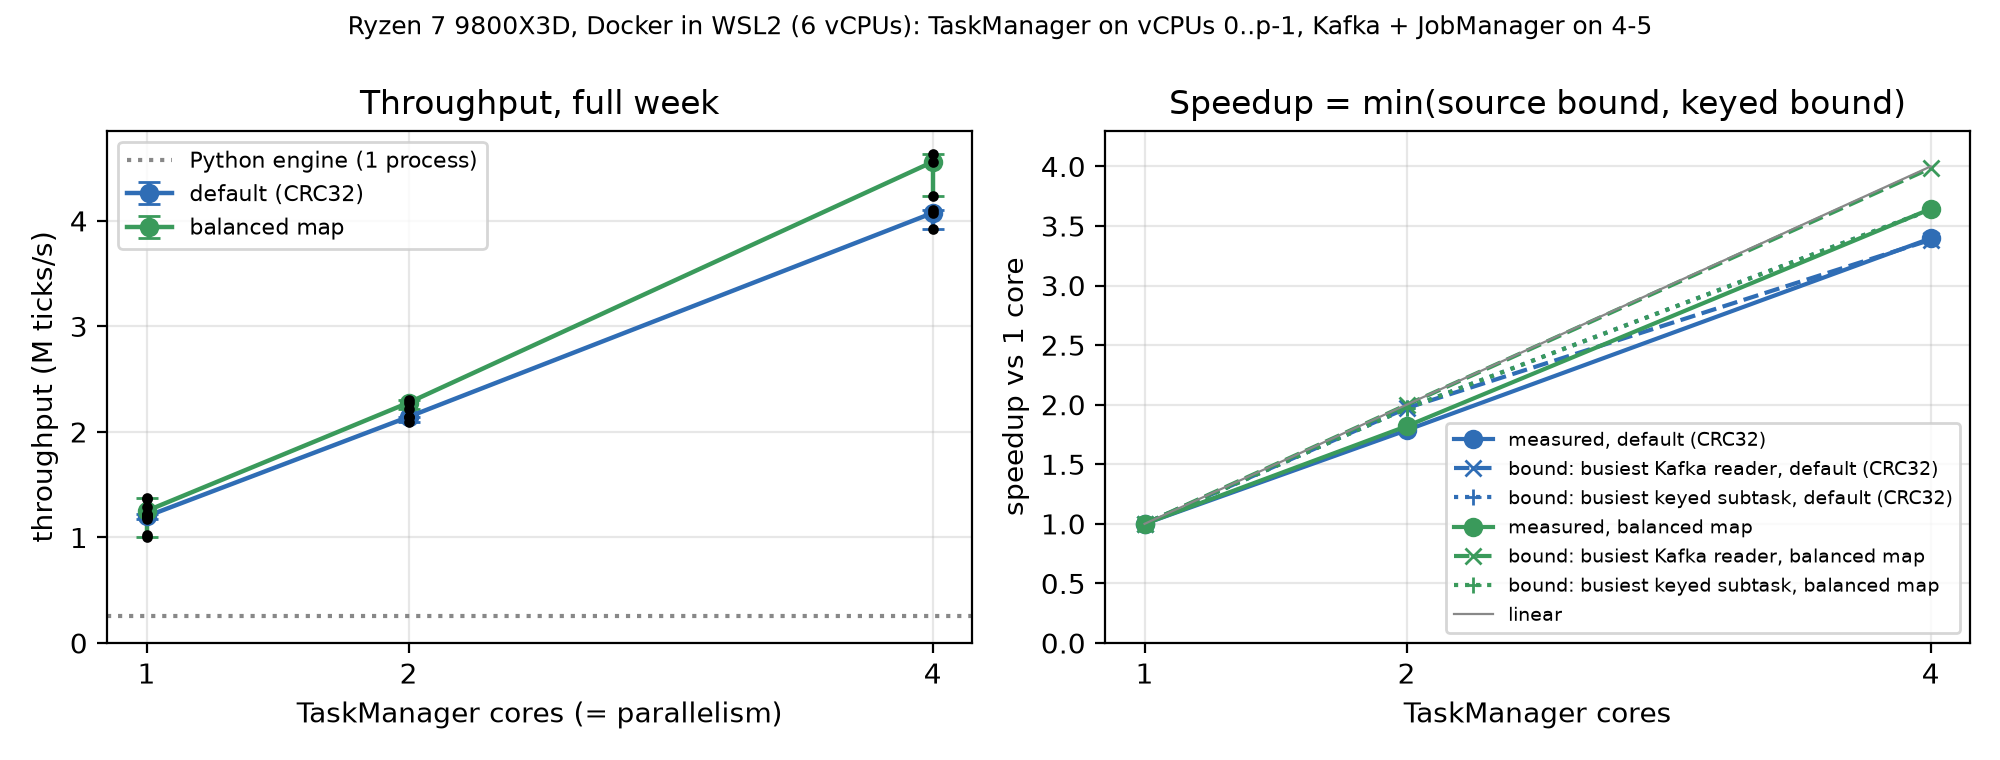
\includegraphics[width=\columnwidth]{figures/throughput_speedup.png}
  \caption{Throughput of the full week (left) and speedup with its two imbalance bounds (right), for
  Kafka's default partitioner and a balanced partition map. Dots are individual runs.}
  \label{fig:throughput}
\end{figure}

\subsection{Scalability}
\emph{Exchanges.} Replaying only Amsterdam (6.0\,M ticks), Amsterdam and Paris (27.4\,M) and all three
exchanges (59.4\,M) at $p=4$ takes 3.1\,s, 10.3\,s and 15.0\,s. The job time grows with the input, and the
larger inputs run at a higher rate (2.0, 2.7 and 4.0\,M ticks/s) because the job's fixed start-up time
weighs less.

\emph{Long tail.} The long-tailed symbol distribution matters only through the imbalance discussed above:
with 4,840 symbols per day, hashing alone keeps the busiest subtask within 10--18\,\% of the mean, and a
count-based partition map removes the source part of it. Hot and rare symbols see the same latency
(Section~\ref{sec:latency}).

\todo{Subscribers 1 to 10,000 (gateway fan-out), if we keep it in the report.}

\subsection{Latency under load}
\label{sec:latency}
We replay the real ticks of 08.11 (11.8\,M) at 100$\times$ to 3000$\times$ real time into a live job ($p=4$,
300\,ms out-of-orderness bound) and measure latency from the moment a window could first close (the first
tick past window end plus the bound on every partition) to the moment its result is written.
Figure~\ref{fig:latency} shows that latency does not grow with load: p50 is 136--185\,ms and p99
224--292\,ms over a 30$\times$ range of input rates. Most of it is Flink's periodic watermark (every 200\,ms);
inside the engine a result takes 7--20\,ms (p50). The 100 most active symbols and the long tail have the same
latency (p50 183 vs 185\,ms at 100$\times$).

\begin{figure}[t]
  \centering
  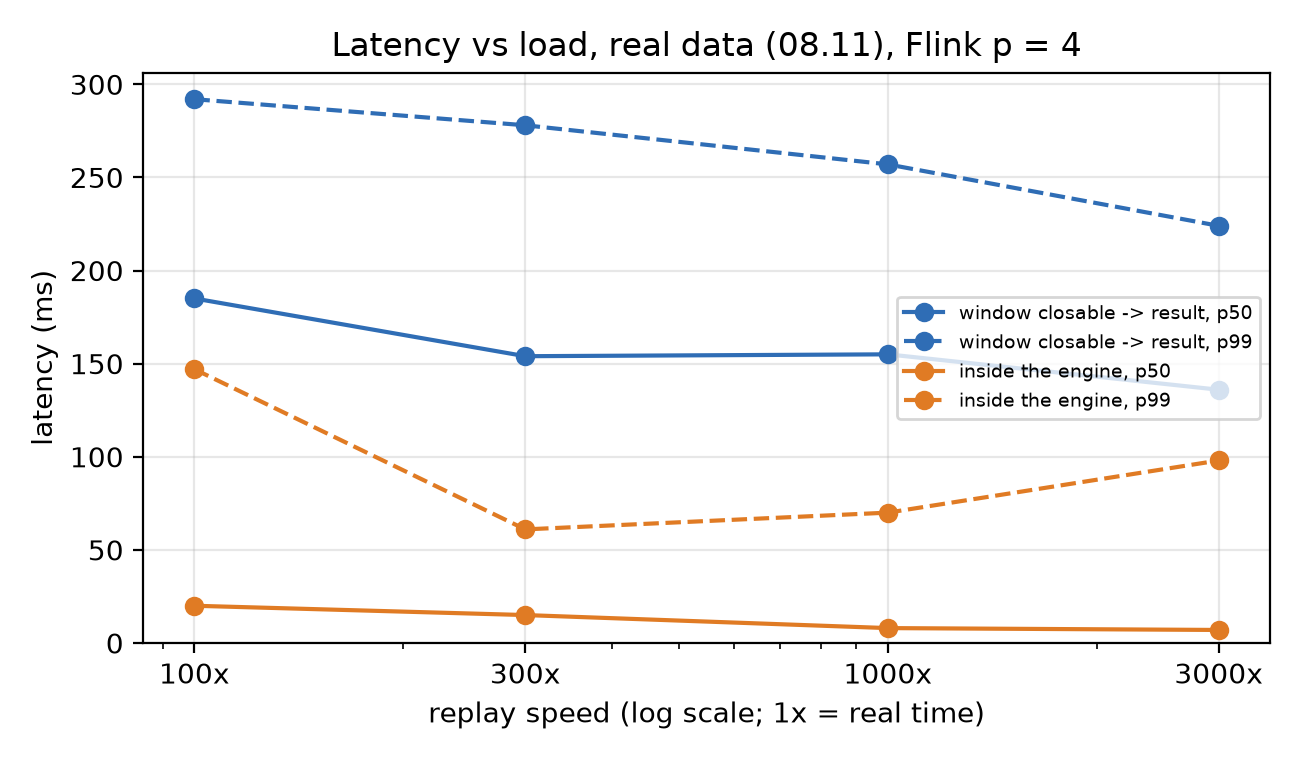
\includegraphics[width=0.9\columnwidth]{figures/latency_vs_speed.png}
  \caption{Latency vs replay speed on the real data of 08.11, $p=4$.}
  \label{fig:latency}
\end{figure}

\subsection{Fault tolerance}
Table~\ref{tab:ft} shows the cost of checkpointing every 10\,s with at-least-once or exactly-once Kafka sinks.
At-least-once costs 2--4\,\%, exactly-once 5--11\,\%; because a full week now drains in 15--30\,s, each run
contains only 2--4 checkpoints (up to 21\,MB each), so these numbers describe short runs. To test recovery,
we killed the TaskManager after 42\,\% (at-least-once) and 36\,\% (exactly-once) of the week at $p=2$. Flink
detected the failure after 10--13\,s, restored the latest checkpoint after 20--21\,s (including the 10\,s
restart delay) and was reading again after 23\,s. Both runs end identical to the reference: exactly-once
with no duplicates for a \texttt{read\_committed} consumer, at-least-once after removing 74,269 duplicate EMA
rows and 39 duplicate advisories, all equal to the rows they repeat.

\begin{table}[t]
  \caption{Throughput (M ticks/s, median of 3 runs) with 10\,s checkpoints.}
  \label{tab:ft}
  \begin{tabular}{lrrr}
    \toprule
    $p$ & none & at-least-once & exactly-once \\
    \midrule
    2 & 2.14 & 2.07 ($-$4\,\%) & 2.04 ($-$5\,\%) \\
    4 & 4.07 & 3.98 ($-$2\,\%) & 3.61 ($-$11\,\%) \\
    \bottomrule
  \end{tabular}
\end{table}

\subsection{Resource use}
The TaskManager uses 91--95\,\% CPU at $p=1$, 176--179\,\% at $p=2$ and 358--369\,\% at $p=4$, so it
keeps 83--92\,\% of each core busy; Kafka (5--13\,\%) and the JobManager (4--9\,\%) stay small. The busiest
operator is the Kafka source with deserialization (81--95\,\% busy), while the keyed window operator
is 58--69\,\% busy on average with no back-pressure. A GPU is not used: per-symbol EMA updates are a few
arithmetic operations on sequential state, so there is nothing to offload.
